%%%% CAPÍTULO 4 - RESULTADOS E DISCUSSÃO
%%
%% Deve descrever detalhadamente os dados obtidos 
%% pelo autor. Normalmente são incluídas ilustrações
%% como: quadros, tabelas, gráficos, etc. Deve efetuar
%% a comparação dos dados obtidos e/ou resultados, com
%% aqueles descritos na revisão de literatura, 
%% incluindo os comentários sobre os estudos de outros
%% autores.

%% Título e rótulo de capítulo (rótulos não devem conter caracteres especiais, acentuados ou cedilha)
\chapter{Resultados e Discussão}
\label{cap:resultadosediscussao}

% Deve descrever detalhadamente os dados obtidos pelo autor. Normalmente são incluídas ilustrações como: quadros, tabelas, gráficos, etc. Deve efetuar a comparação dos dados obtidos e/ou resultados, com aqueles descritos na revisão de literatura, incluindo os comentários sobre os estudos de outros autores.


\ric{Vamos organizar o capítulo da seguinte forma:}

\begin{enumerate}
    \item Análise exploratória: resultados estatísticos (visualizações) que permitam caracterizar de forma geral a base de dados utilizada;
    
    \item Operação da rede de transporte: resultados obtidos do uso de grafos temporais na caracterização da operação atual da rede de transporte de Curitiba;
    
    \item Integração temporal: resultados do estudo de uma integração temporal na rede de transporte de Curitiba
\end{enumerate}

\section{Análise exploratória}

Os resultados foram obtidos para o período de  01/03/2019 a 30/06/2019, tendo sido coletados 33 Gigabytes de dados, com 293.390.175 registros de geolocalização dos 1708 ônibus e 364 linhas em operação. É importante destacar que cerca de 6\% dos registros de geolocalização fornecidos estavam duplicados e foram removidos no processamento da base. A frequência média de posicionamento dos veículos é de 10 segundos.
Este volume de dados gerou, após a transformação para o banco de dados de grafo do Neo4j, 26.869.679 vértices e 93.082.943 arestas sendo necessárias cerca de 12 horas de processamento em uma computador com processador i7 10ª geração e 32GB memória RAM.

As Figuras~\ref{fig:eventos_crus}, \ref{fig:veículosregistrados} e \ref{fig:linhasregistradas}  apresentam algumas informações encontradas na base de dados disponibilizada.

\ric{A Figura~\ref{fig:eventos_crus} mostra o número de eventos de geolocalização coletados dos ônibus por dia, no período considerado. Este número deveria ser aproximadamente igual, execeto para finais de semana. Porém, nota-se que existe uma grande variação nos dados coletedos por dia. Isso pode ser devido a problemas de comunicação... Assim, as análises feitas neste trabalho consideram apenas dias da semana que possuem um volumes de dados similares. Aqui é o ponto para justificar as escolha de determinados dias para a análise.}
% A Figura~\ref{fig:eventos_crus} representa a distribuição de eventos de geolocalização ao longo do período da base coletada. Pode-se verificar uma grande variância no número de eventos de posicionamento.
\begin{figure}
\centering
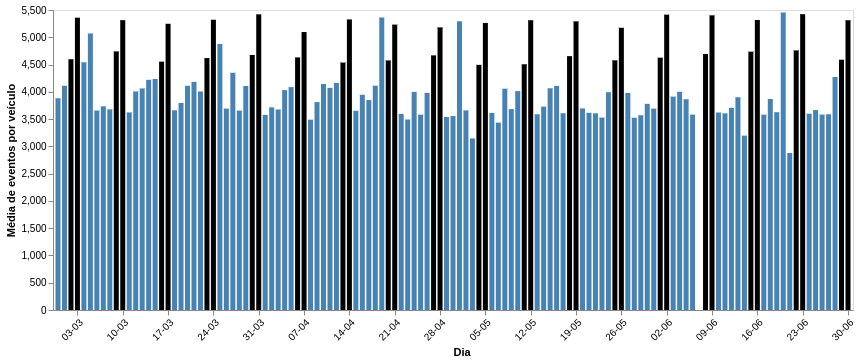
\includegraphics[width=.9\textwidth]{Capitulo4/img/eventos_por_veiculo.png}
\caption{Número médio de eventos por veículo no período de 01/03/2019 à 30/06/2019.}
\label{fig:eventos_crus}
\end{figure}


% A Tabela~\ref{tab:neo} mostra estatísticas do banco de dados construído no Neo4j, com informações sobre o transporte coletivo de Curitiba coletados durante o período de 01/03/2019 a 30/06/2019.

% \begin{table}[h]
%     \caption{Estatísticas do banco de dados de grafo construído.}
%     \label{tab:neo}
%     \centering
%     \begin{tabular}{ccc} 
%         \hline
%         No. vértices & No. de arestas\\
%         \hline
%         26.869.679 & 93.082.943 \\
%         \hline  
%     \end{tabular}
% \end{table}


A Figura~\ref{fig:veículosregistrados} apresenta a distribuição de veículos ao longo do tempo cujo apresentaram eventos de geolocalização na base coletada.

\begin{figure}
\centering
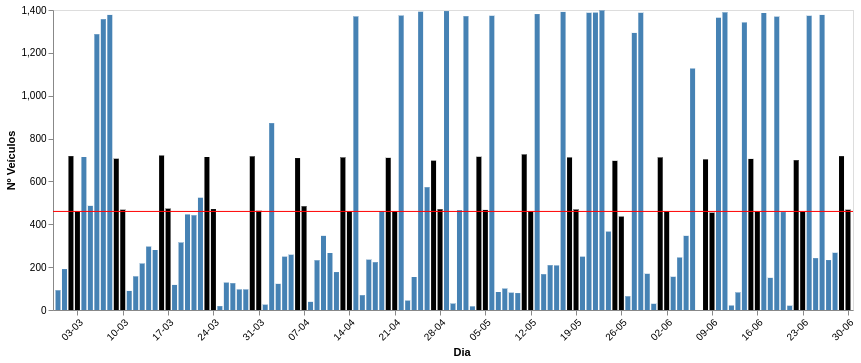
\includegraphics[width=.9\textwidth]{Capitulo4/img/veiculos.png}
\caption{Número de veículos registrados no período de 01/03/2019 à 30/06/2019.}
\label{fig:veículosregistrados}
\end{figure}


A Figura~\ref{fig:linhasregistradas} apresenta a distribuição de linhas ao longo do tempo que tiveram veículos emitindo eventos de geolocalização na base coletada.
\begin{figure}
\centering
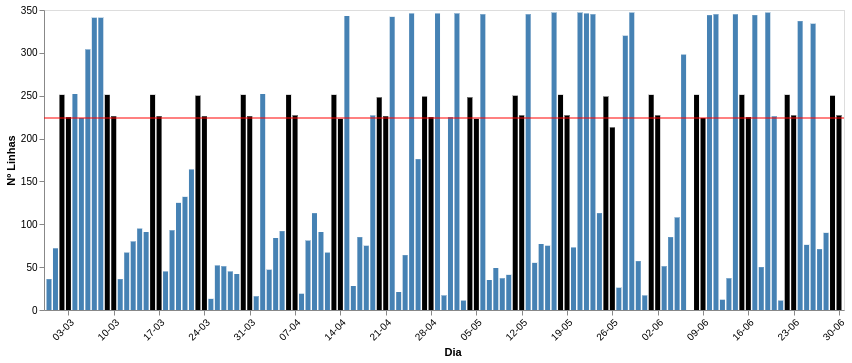
\includegraphics[width=.9\textwidth]{Capitulo4/img/linhas-registradas.png}
\caption{Número de linhas registrados no período de 01/03/2019 à 30/06/2019.}
\label{fig:linhasregistradas}
\end{figure}




\section{Operação da rede de transporte}

% \ric{Resultados que podem ser derivados da modelagem proposta usando grafos temporais. Mais ou menos na linha do artigo do Courb.}

% {plotar rede estática}

\ric{Não deveria aparecer aqui os detalhes de como foram geradas as séries temporais de eventos em cada ponto de ônibus?}

\begin{figure}
\centering
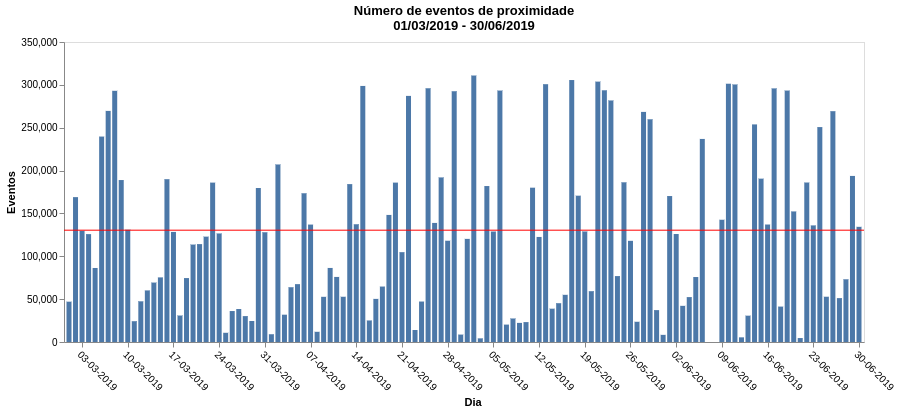
\includegraphics[width=.9\textwidth]{Capitulo4/img/eventos_proximidade.png}
\caption{Número de eventos de proximidade coletados no período de 01/03/2019 à 30/06/2019.}
\label{fig:eventos-de-proximidade}
\end{figure}


A Figura~\ref{fig:eventosproximidade-110126} apresenta a distribuição de eventos de proximidade ao longo do tempo para o ponto 110126.
\begin{figure}
\centering
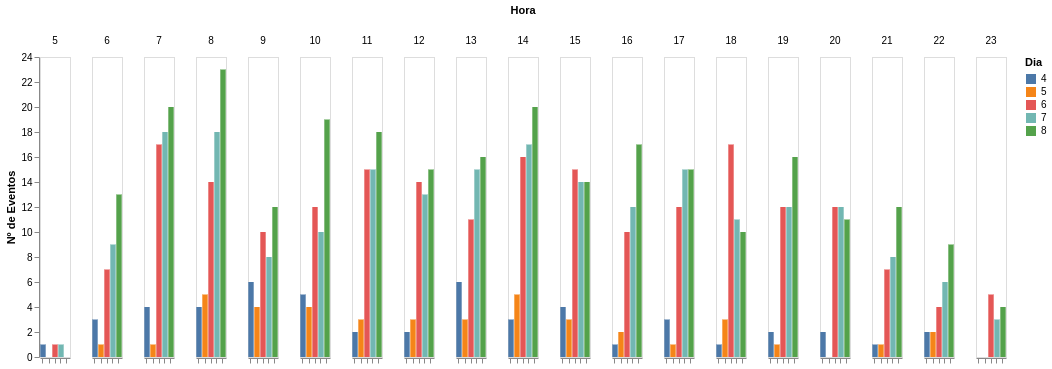
\includegraphics[width=.9\textwidth]{Capitulo4/img/eventos-proximidade-110126.png}
\caption{Número de eventos de proximidade registrados no período de 04/03/2019 à 08/03/2019 para o ponto 110126}
\label{fig:eventosproximidade-110126}
\end{figure}



% \ric{Figuras de centralidade parecem ser melhor apresentadas em mapas, onde se pode ver a localização dos pontos considerados.}

% \begin{figure}
% \centering
% 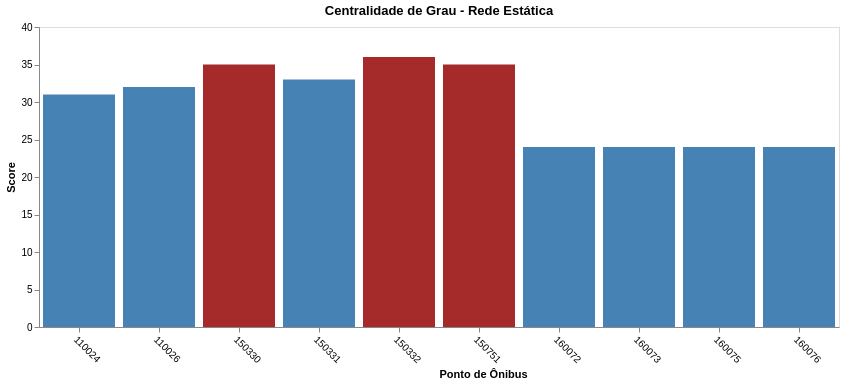
\includegraphics[width=.9\textwidth]{Capitulo4/img/centralidade-grau.png}
% \caption{Centralidade de grau da rede estática.}
% \label{fig:centralidade-grau}
% \end{figure}

\begin{figure}[!h]
\caption{Centralidade de grau e pagerank da rede estática.}
\label{fig:map-centralidade-grau-estatica.png}
\centering
\subfloat[Centralidade de grau.]{
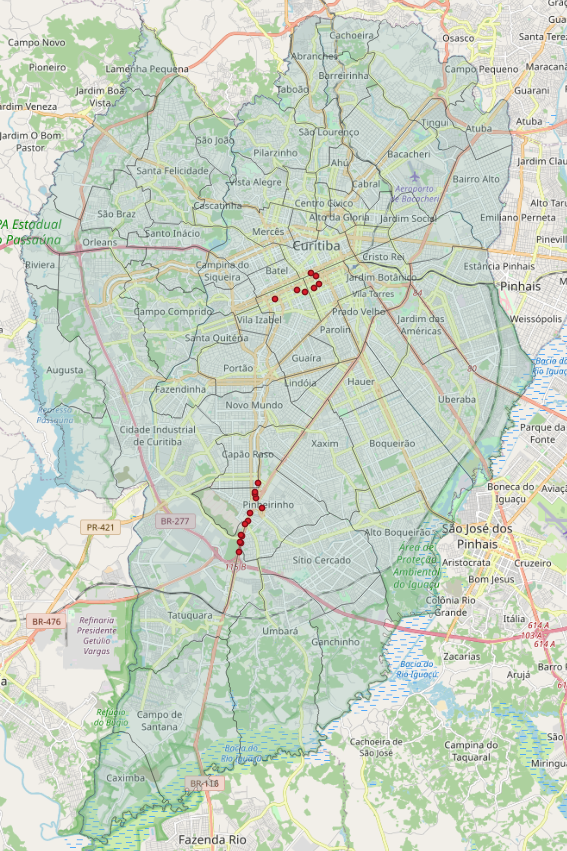
\includegraphics[width=.4\textwidth]{Capitulo4/img/rede-estatica/map-centralidade-grau.png}
}
\quad
\subfloat[Pagerank.]{
\label{fig:map-pagerank-estatica.png}
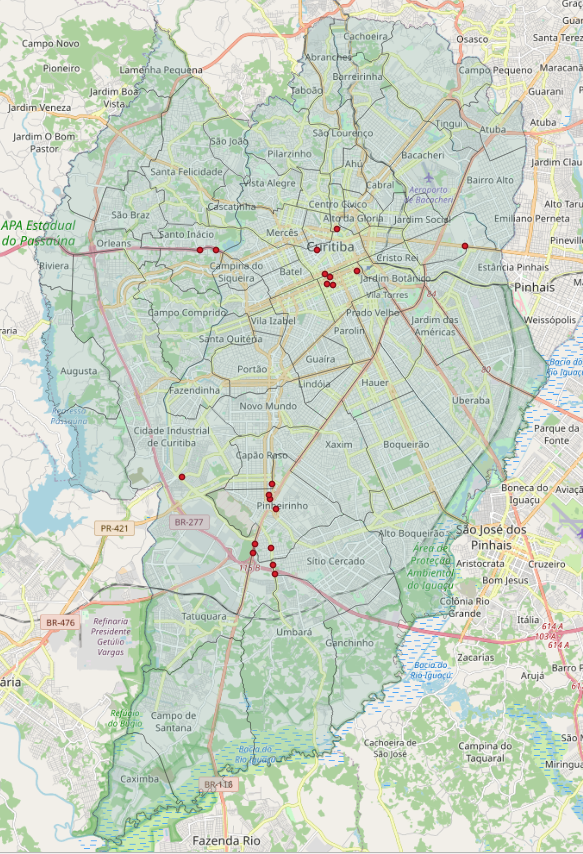
\includegraphics[width=.4\textwidth]{Capitulo4/img/rede-estatica/map-pagerank.png}
}
\end{figure}



% \begin{figure}
% \centering
% 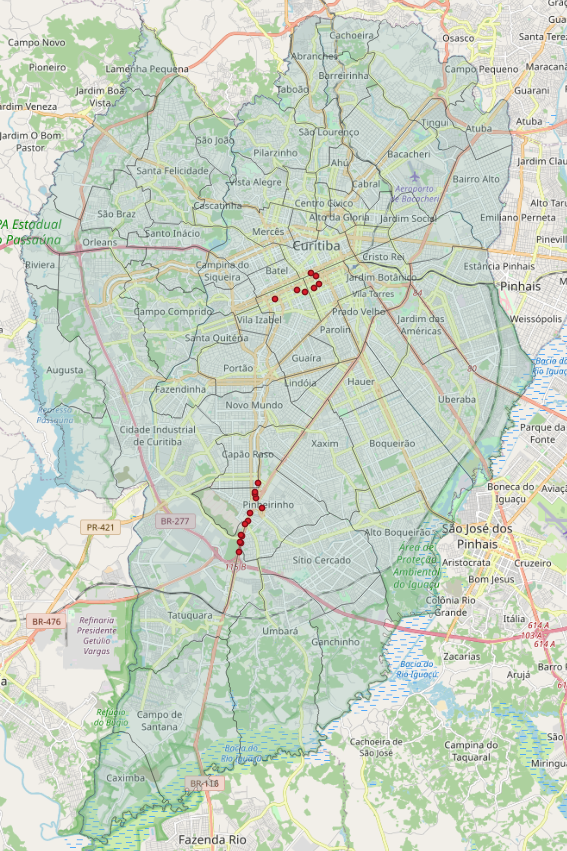
\includegraphics[width=.4\textwidth]{Capitulo4/img/rede-estatica/map-centralidade-grau.png}
% \caption{Centralidade de grau da rede estática.}
% \label{fig:map-centralidade-grau-estatica.png}
% \end{figure}

\begin{table}[htb]
    \caption{Pontos de ônibus com maior centralidade de grau da rede estática.}
    \label{tab:centralidade-grau-rede-estatica}
    \centering
    \footnotesize
    \begin{tabular}{clc} 
        \hline
        Ponto (ID) & Endereço & Centralidade grau \\
        \hline
       \texttt{150332} &                 Rua Leon Nicolas, 2081 - Capão Raso &  36.00 \\
       \textbf{\texttt{150751}} &            Av. Winston Churchill, 2677 - Capão Raso &  35.00 \\
       \textbf{\texttt{150330}} &            Av. Winston Churchill, 2546 - Capão Raso &  35.00 \\
       \texttt{150331} &            Av. Winston Churchill, 2472 - Capão Raso &  33.00 \\
       \textbf{\texttt{110026}} &                    Rua Alferes Poli, 400 - Rebouças &  32.00 \\
       \textbf{\texttt{110024}} &                    Rua Alferes Poli, 787 - Rebouças &  31.00 \\
       \texttt{160076} &  Rodovia BR476 - Pista Lateral, 20227 - Pinheirinho &  24.00 \\
       \texttt{160075} &                  Rodovia BR476, 20917 - Pinheirinho &  24.00 \\
       \textbf{\texttt{160073}} &                  Rodovia BR476, 21251 - Pinheirinho &  24.00 \\
       \textbf{\texttt{160072}} &            Rodovia BR476, 21283 - Cidade Industrial &  24.00 \\
       \textbf{\texttt{160244}} &                Rua Emanoel Voluz, 284 - Pinheirinho &  23.00 \\
       \texttt{170121} &  Rodovia BR476 - Pista Lateral, 20916 - Pinheirinho &  23.00 \\
       \textbf{\texttt{110022}} &        Rua Vinte e Quatro de Maio, 280-350 - Centro &  22.00 \\
       \texttt{160438} &  Rodovia BR476 - Pista Lateral, 20228 - Pinheirinho &  21.00 \\
       \texttt{160078} &         Rodovia BR476 - Pista Lateral - Pinheirinho &  21.00 \\
       \texttt{160074} &            Rodovia BR476, 21152 - Cidade Industrial &  21.00 \\
       \texttt{110211} &           Av. Pres. Getulio Vargas, 1309 - Rebouças &  20.00 \\
       \texttt{150631} &                       Av. Iguaçu, 1788 - Água Verde &  20.00 \\
       \texttt{150634} &                       Av. Iguaçu, 2612 - Água Verde &  20.00 \\
       \texttt{110210} &           Av. Pres. Getúlio Vargas, 1708 - Rebouças &  20.00 \\
        
        \hline  
    \end{tabular}
\end{table}


% \begin{table}[htb]
%     \caption{Pontos de maior centralidade de grau da rede estática.}
%     \label{tab:centralidade-grau-rede-estatica}
%     \centering
%     \footnotesize
%     \begin{tabular}{p{1.0cm}p{7.0cm}p{2.5cm}p{2.5cm}p{1.0cm} } 
%         \hline
%         Número & Endereço & latitude & longitude & Score \\
%         \hline
        
%       \texttt{150332} &                 Rua Leon Nicolas, 2081 - Capão Raso &  -25.515159644727 &  -49.294443608469 &  36.00 \\
%       \texttt{150751} &            Av. Winston Churchill, 2677 - Capão Raso &  -25.520731874323 &  -49.295383384725 &  35.00 \\
%       \texttt{150330} &            Av. Winston Churchill, 2546 - Capão Raso &  -25.519229941942 &  -49.295454463264 &  35.00 \\
%       \texttt{150331} &            Av. Winston Churchill, 2472 - Capão Raso &  -25.518348864079 &   -49.29566769888 &  33.00 \\
%       \texttt{110026} &                    Rua Alferes Poli, 400 - Rebouças &  -25.440705808683 &  -49.271456482887 &  32.00 \\
%       \texttt{110024} &                    Rua Alferes Poli, 787 - Rebouças &  -25.443478176732 &  -49.270140950921 &  31.00 \\
%       \texttt{160076} &  Rodovia BR476 - Pista Lateral, 20227 - Pinheirinho &   -25.52887878983 &  -49.298525743551 &  24.00 \\
%       \texttt{160075} &                  Rodovia BR476, 20917 - Pinheirinho &  -25.534129437556 &  -49.300630712105 &  24.00 \\
%       \texttt{160073} &                  Rodovia BR476, 21251 - Pinheirinho &  -25.536584739941 &  -49.301261031223 &  24.00 \\
%       \texttt{160072} &            Rodovia BR476, 21283 - Cidade Industrial &  -25.539911210059 &  -49.301985597553 &  24.00 \\
%       \texttt{160244} &                Rua Emanoel Voluz, 284 - Pinheirinho &  -25.524017075104 &  -49.292992119479 &  23.00 \\
%       \texttt{170121} &  Rodovia BR476 - Pista Lateral, 20916 - Pinheirinho &   -25.53378939418 &  -49.301047795606 &  23.00 \\
%       \texttt{110022} &        Rua Vinte e Quatro de Maio, 280-350 - Centro &  -25.439756734365 &  -49.273240017786 &  22.00 \\
%       \texttt{160438} &  Rodovia BR476 - Pista Lateral, 20228 - Pinheirinho &  -25.529798854542 &  -49.299592186508 &  21.00 \\
%       \texttt{160078} &         Rodovia BR476 - Pista Lateral - Pinheirinho &  -25.525878471402 &  -49.297614519014 &  21.00 \\
%       \texttt{160074} &            Rodovia BR476, 21152 - Cidade Industrial &  -25.536449209528 &  -49.301535957647 &  21.00 \\
%       \texttt{110211} &           Av. Pres. Getulio Vargas, 1309 - Rebouças &  -25.445197981519 &  -49.272273809856 &  20.00 \\
%       \texttt{150631} &                       Av. Iguaçu, 1788 - Água Verde &  -25.445710238874 &  -49.278719158119 &  20.00 \\
%       \texttt{150634} &                       Av. Iguaçu, 2612 - Água Verde &  -25.448942375096 &  -49.287531555838 &  20.00 \\
%       \texttt{110210} &           Av. Pres. Getúlio Vargas, 1708 - Rebouças &  -25.446516767314 &   -49.27578884477 &  20.00 \\
        
%         \hline  
%     \end{tabular}
% \end{table}


% \begin{figure}
% \centering
% 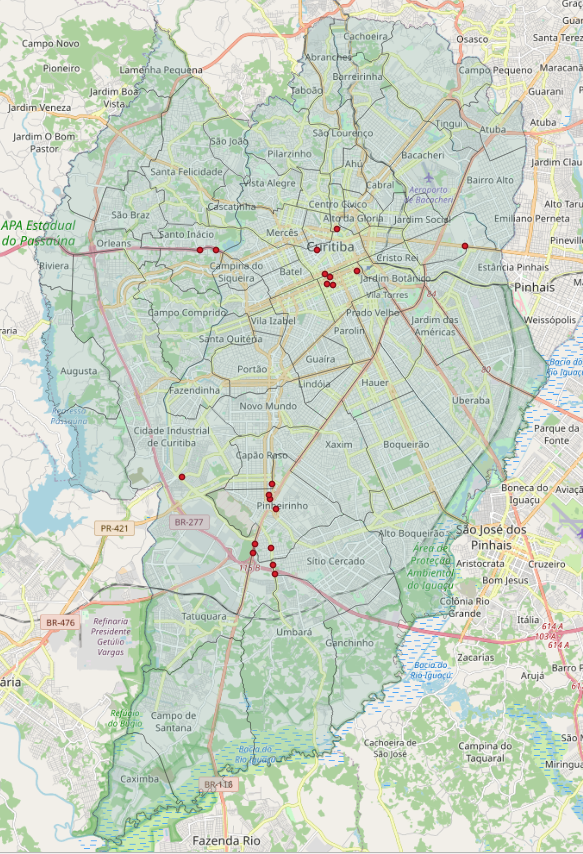
\includegraphics[width=.4\textwidth]{Capitulo4/img/rede-estatica/map-pagerank.png}
% \caption{Pagerank da rede estática.}
% \label{fig:map-pagerank-estatica.png}
% \end{figure}



\begin{table}[htb]
    \caption{Pontos de ônibus com maior pagerank da rede estática.}
    \label{tab:pagerank-rede-estatica}
    \centering
    \footnotesize
    \begin{tabular}{clc} 
        \hline
        Ponto (ID) & Endereço & Pagerank \\
        \hline
        \textbf{\texttt{150751}} &      Av. Winston Churchill, 2677 - Cap?o Raso &   5.69 \\
        \texttt{110126} &    Rua Heitor S de Franca, 93 - Centro Civico &   5.27 \\
        \textbf{\texttt{160244}} &          Rua Emanoel Voluz, 284 - Pinheirinho &   5.00 \\
        \textbf{\texttt{150330}} &      Av. Winston Churchill, 2546 - Cap?o Raso &   4.89 \\
        \texttt{110016} &                Rua Cruz Machado, 301 - Centro &   4.29 \\
        \texttt{150332} &           Rua Leon Nicolas, 2081 - Cap?o Raso &   4.26 \\
        \textbf{\texttt{110024}} &              Rua Alferes Poli, 787 - Reboucas &   4.04 \\
        \textbf{\texttt{110026}} &              Rua Alferes Poli, 400 - Reboucas &   3.74 \\
        \textbf{\texttt{160072}} &      Rodovia BR476, 21283 - Cidade Industrial &   3.72 \\
        \texttt{160145} &       Rua Nicola Pellanda, 1719 - Pinheirinho &   3.71 \\
        \textbf{\texttt{110022}}&  Rua Vinte e Quatro de Maio, 280-350 - Centro &   3.70 \\
        \texttt{130215} &  Av. Victor Ferreira do Amaral, 1447 - Tarum? &   3.63 \\
        \texttt{110147} &        Rua Conselheiro Laurindo, 1264- Centro &   3.56 \\
        \texttt{160327} &       Rua Nicola Pellanda, 2091 - Pinheirinho &   3.44 \\
        \texttt{180077} &     Rua Pedro Gusso, 4311 - Cidade Industrial &   3.42 \\
        \textbf{\texttt{160073}} &            Rodovia BR476, 21251 - Pinheirinho &   3.37 \\
        \texttt{190199} &  Marginal Rodovia BR- 277, 926 - Santo Inacio &   3.36 \\
        \texttt{110208} &                   Av. Iguacu, 1184 - Reboucas &   3.30 \\
        \texttt{160141} &       Rua Nicola Pellanda, 1031 - Pinheirinho &   3.29 \\
        \texttt{190198} &  Marginal Rodovia BR- 277, 926 - Santo Inacio &   3.28 \\
        \hline  
    \end{tabular}
\end{table}


% \begin{table}[htb]
%     \caption{Pontos de ônibus com maior pagerank da rede estática.}
%     \label{tab:pagerank-rede-estatica}
%     \centering
%     \footnotesize
%     \begin{tabular}{p{1.0cm}p{4.0cm}p{3.0cm}p{3.0cm}p{3.0cm} } 
%         \hline
%         Número & Endereço & latitude & longitude & Score \\
%         \hline
%         \texttt{150751} &      Av. Winston Churchill, 2677 - Cap?o Raso &  -25.520731874323 &  -49.295383384725 &   5.69 \\
%         \texttt{110126} &    Rua Heitor S de Franca, 93 - Centro Civico &  -25.423318109898 &  -49.268572186508 &   5.27 \\
%         \texttt{160244} &          Rua Emanoel Voluz, 284 - Pinheirinho &  -25.524017075104 &  -49.292992119479 &   5.00 \\
%         \texttt{150330} &      Av. Winston Churchill, 2546 - Cap?o Raso &  -25.519229941942 &  -49.295454463264 &   4.89 \\
%         \texttt{110016} &                Rua Cruz Machado, 301 - Centro &  -25.430894327324 &  -49.276454032606 &   4.29 \\
%         \texttt{150332} &           Rua Leon Nicolas, 2081 - Cap?o Raso &  -25.515159644727 &  -49.294443608469 &   4.26 \\
%         \texttt{110024} &              Rua Alferes Poli, 787 - Reboucas &  -25.443478176732 &  -49.270140950921 &   4.04 \\
%         \texttt{110026} &              Rua Alferes Poli, 400 - Reboucas &  -25.440705808683 &  -49.271456482887 &   3.74 \\
%         \texttt{160072} &      Rodovia BR476, 21283 - Cidade Industrial &  -25.539911210059 &  -49.301985597553 &   3.72 \\
%         \texttt{160145} &       Rua Nicola Pellanda, 1719 - Pinheirinho &  -25.544221680924 &     -49.294155271 &   3.71 \\
%         \texttt{110022} &  Rua Vinte e Quatro de Maio, 280-350 - Centro &  -25.439756734365 &  -49.273240017786 &   3.70 \\
%         \texttt{130215} &  Av. Victor Ferreira do Amaral, 1447 - Tarum? &  -25.429560368269 &  -49.217533947176 &   3.63 \\
%         \texttt{110147} &        Rua Conselheiro Laurindo, 1264- Centro &  -25.438529389521 &  -49.260738969988 &   3.56 \\
%         \texttt{160327} &       Rua Nicola Pellanda, 2091 - Pinheirinho &   -25.54745116804 &  -49.293365360445 &   3.44 \\
%         \texttt{180077} &     Rua Pedro Gusso, 4311 - Cidade Industrial &  -25.512755963766 &  -49.330335189755 &   3.42 \\
%         \texttt{160073} &            Rodovia BR476, 21251 - Pinheirinho &  -25.536584739941 &  -49.301261031223 &   3.37 \\
%         \texttt{190199} &  Marginal Rodovia BR- 277, 926 - Santo Inacio &  -25.431003976097 &  -49.316830961971 &   3.36 \\
%         \texttt{110208} &                   Av. Iguacu, 1184 - Reboucas &  -25.443296676303 &  -49.272462905592 &   3.30 \\
%         \texttt{160141} &       Rua Nicola Pellanda, 1031 - Pinheirinho &  -25.538179630971 &  -49.294743263316 &   3.29 \\
%         \texttt{190198} &  Marginal Rodovia BR- 277, 926 - Santo Inacio &  -25.430958050444 &  -49.322961066418 &   3.28 \\
%         \hline  
%     \end{tabular}
% \end{table}


\begin{figure}[!h]
\caption{Centralidades de intermediação e proximidade da rede estática.}
\label{fig:map-betweeness-rede-estatica}
\centering
\subfloat[Centralidade de intermediação.]{
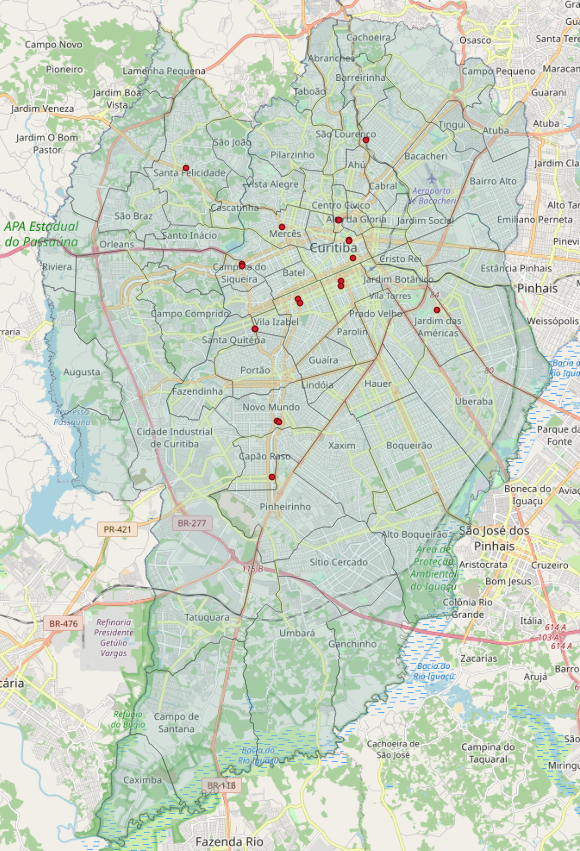
\includegraphics[width=.4\textwidth]{Capitulo4/img/rede-estatica/map-centralidade-intermediacao.png}
}
\quad
\subfloat[Centralidade de proximidade.]{
\label{fig:map-closeness-rede-estatica}
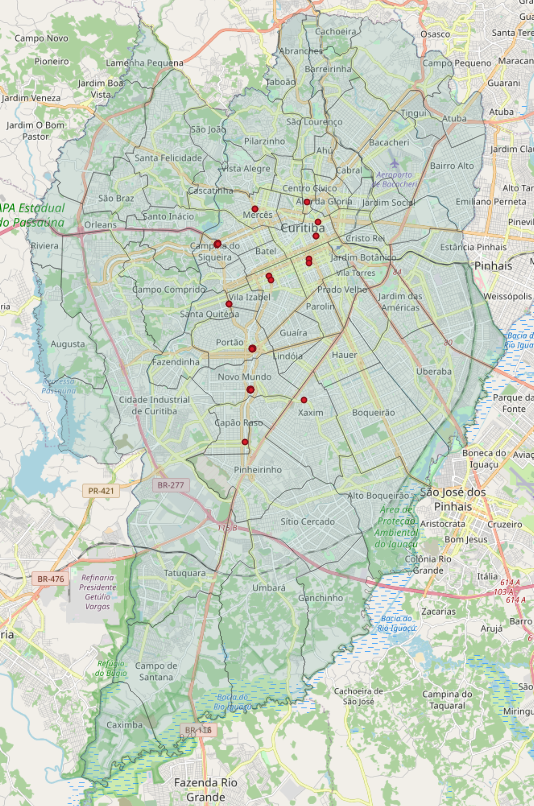
\includegraphics[width=.4\textwidth]{Capitulo4/img/rede-estatica/map-centralidade-proximidade.png}
}
\end{figure}


% \begin{figure}
% \centering
% 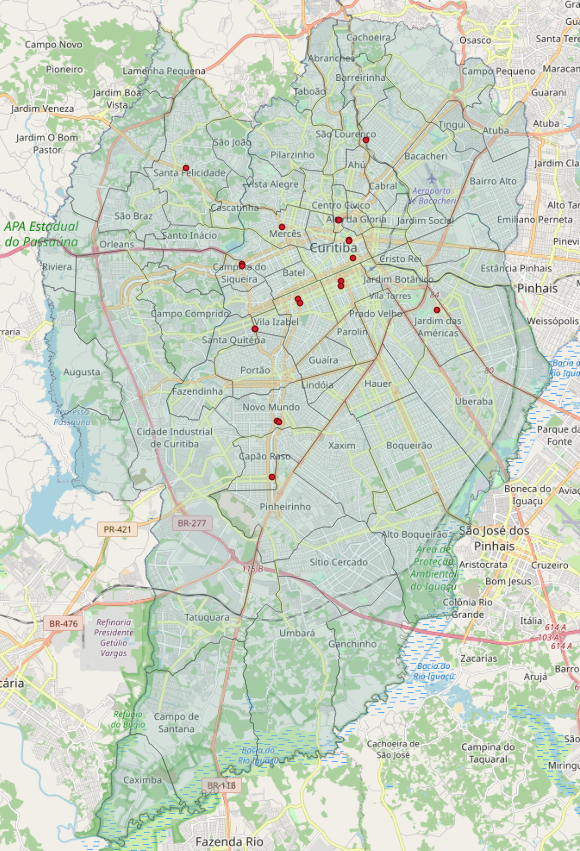
\includegraphics[width=.4\textwidth]{Capitulo4/img/rede-estatica/map-centralidade-intermediacao.png}
% \caption{Centralidade de Intermediação}
% \label{fig:map-betweeness-rede-estatica}
% \end{figure}
   



\begin{table}[htb]
    \caption{Pontos de maior Centralidade de Intermediação da rede estática.}
    \label{tab:centralidade-grau-rede-estatica}
    \centering
    \footnotesize
    \begin{tabular}{p{1.0cm}p{9.0cm}p{3.0cm} } 
        \hline
        Número & Endereço & Score \\
        \hline
        \texttt{109093} &       Terminal Capão Raso - 023 - Inter 2 (Anti-Horário) / 508-Sitio Cercado (Anti-Horário)  & 6858923.35 \\
        \texttt{109003} &                                                            Estacão Tubo Água Verde / Iguaçu  & 6816043.76 \\
        \texttt{109023} &                                                             Estacão Tubo Comendador Fontana  & 5414297.56 \\
        \texttt{109067} &                                                                 Estacão Tubo Santa Quitéria  & 5393530.56 \\
        \texttt{109004} &                                                                            Estacão Tubo Ahu  & 5337840.08 \\
        \texttt{109073} &                                                            Estacão Tubo Westphalen / Iguaçu  & 5288723.46 \\
        \texttt{109066} &                                                                 Estacão Tubo Santa Quitéria  & 5045554.12 \\
        \texttt{109018} &                                                                Estacão Tubo Circulo Militar  & 4838282.83 \\
        \texttt{109019} &                                                                Estacão Tubo Circulo Militar  & 4782184.83 \\
        \texttt{109098} &                                 Terminal Pinheirinho - 508 - Sitio Cercado (Anti - Horário)  & 4580919.38 \\
        \texttt{109167} &  Terminal Campina do Siqueira - 023 - Inter 2 (Anti-Horário) - 024 - C.Raso - Camp.Siqueira  & 4519411.68 \\
        \texttt{109121} &                             Terminal Santa Felicidade - 307 - Santa Felicidade/ Bairro Alto  & 4132317.46 \\
        \texttt{109034} &                                                            Estacão Tubo Jardim das Américas  & 4006981.03 \\
        \texttt{109022} &                                                             Estacão Tubo Comendador Fontana  & 3988692.54 \\
        \texttt{109125} &                                      Terminal Campina do Siqueira - 022 - Inter 2 (Horário)  & 3954715.60 \\
        \texttt{109046} &                                                                         Estacão Tubo Merces  & 3788812.85 \\
        \texttt{109002} &                                                    Estacão Tubo Água Verde / Getúlio Vargas  & 3719017.52 \\
        \texttt{109074} &                                                    Estacão Tubo Westphalen / Getúlio Vargas  & 3718993.52 \\
        \texttt{109030} &                                                                      Estacão Tubo Guadalupe  & 3718969.52 \\
        \texttt{109097} &                       Terminal Capão Raso - 507 - Sitio Cercado(H) - 610-S.Cercado / C.Raso  & 3714691.73 \\
        \hline  
    \end{tabular}
\end{table}


% \begin{figure}
% \centering
% 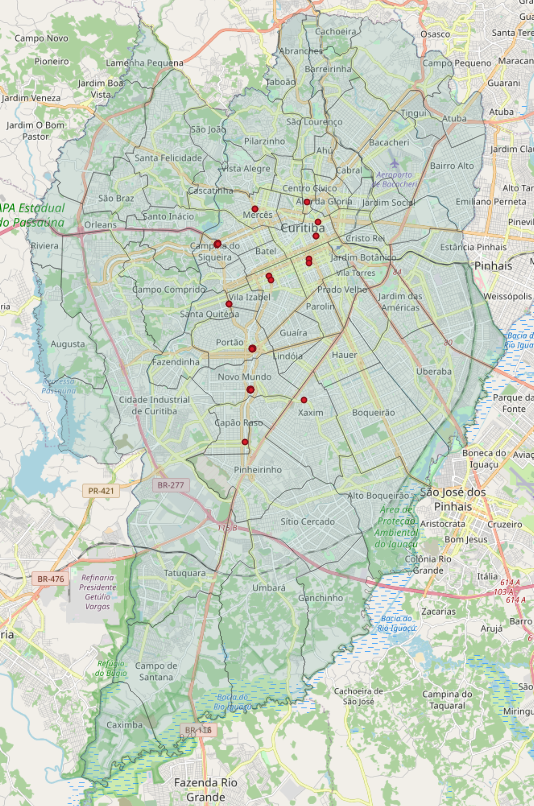
\includegraphics[width=.4\textwidth]{Capitulo4/img/rede-estatica/map-centralidade-proximidade.png}
% \caption{Centralidade de Proximidade}
% \label{fig:map-closeness-rede-estatica}
% \end{figure}
   

\begin{table}[htb]
    \caption{Pontos de maior Centralidade de Proximidade da rede estática.}
    \label{tab:centralidade-grau-rede-estatica}
    \centering
    \footnotesize
    \begin{tabular}{p{1.0cm}p{9.0cm}p{3.0cm} } 
        \hline
        Número & Endereço & Score \\
        \hline
            \texttt{109093} &          Terminal Cap?o Raso - 023 - Inter 2 (Anti-Horario) / 508-Sitio Cercado (Anti-Horario)  & 0.0850 \\
           \texttt{109003} &                                                               Estac?o Tubo Agua Verde / Iguacu  & 0.0848 \\
           \texttt{109167} &     Terminal Campina do Siqueira - 023 - Inter 2 (Anti-Horario) - 024 - C.Raso - Camp.Siqueira  & 0.0841 \\
           \texttt{109125} &                                         Terminal Campina do Siqueira - 022 - Inter 2 (Horario)  & 0.0839 \\
           \texttt{109066} &                                                                    Estac?o Tubo Santa Quiteria  & 0.0839 \\
           \texttt{109067} &                                                                    Estac?o Tubo Santa Quiteria  & 0.0838 \\
           \texttt{109002} &                                                       Estac?o Tubo Agua Verde / Getulio Vargas  & 0.0835 \\
           \texttt{109089} &                                                 Terminal Port?o - 023 - Inter 2 (Anti-Horario)  & 0.0834 \\
           \texttt{109091} &                                                      Terminal Port?o - 022 - Inter 2 (Horario)  & 0.0834 \\
           \texttt{109097} &                          Terminal Cap?o Raso - 507 - Sitio Cercado(H) - 610-S.Cercado / C.Raso  & 0.0831 \\
           \texttt{109095} &                                                  Terminal Cap?o Raso - 022 - Inter 2 (Horario)  & 0.0830 \\
           \texttt{109073} &                                                               Estac?o Tubo Westphalen / Iguacu  & 0.0824 \\
           \texttt{109046} &                                                                            Estac?o Tubo Merces  & 0.0819 \\
           \texttt{109090} &                                                   Terminal Port?o - 700 - Pinheirinho / Cabral  & 0.0817 \\
           \texttt{109019} &                                                                   Estac?o Tubo Circulo Militar  & 0.0814 \\
           \texttt{109047} &                                                                            Estac?o Tubo Merces  & 0.0814 \\
           \texttt{104804} &                                 Terminal Cap?o Raso - 502 - Circular Sul (H) - 603-Pinheirinho  & 0.0812 \\
           \texttt{109074} &                                                       Estac?o Tubo Westphalen / Getulio Vargas  & 0.0811 \\
           \texttt{109094} &                               Terminal Cap?o Raso - 210 - CIC/ Cabral - 606 - Ctba / Araucaria  & 0.0809 \\
           \texttt{109096} &                                                       Terminal Cap?o Raso - 210 - CIC / Cabral  & 0.0809 \\
           \texttt{109077} &                                                                             Estac?o Tubo Xaxim  & 0.0809 \\
           \texttt{109098} &                                    Terminal Pinheirinho - 508 - Sitio Cercado (Anti - Horario)  & 0.0808 \\
           \texttt{109124} &                                  Terminal Campina do Siqueira - 304 - Pinhais / Campo Comprido  & 0.0808 \\
           \texttt{104506} &                            Terminal Campina do Siqueira - 021 - Interbairros II (Anti-Horario)  & 0.0807 \\
           \texttt{109126} &                                  Terminal Campina do Siqueira - 304 - Pinhais / Campo Comprido  & 0.0807 \\
           \texttt{109092} &                                                   Terminal Port?o - 700 - Pinheirinho / Cabral  & 0.0804 \\
           \texttt{109023} &                                                                Estac?o Tubo Comendador Fontana  & 0.0803 \\
           \texttt{105802} &  Terminal Port?o-202-Cabral/C.Raso-203-Sta.Candida/C.Raso-603-Pinheirinho-602-Circular Sul(AH)  & 0.0802 \\
           \texttt{109028} &                    Terminal Guadalupe - 702 - Caiua / Cachoeira - X36 - Fazendinha / Guadalupe  & 0.0802 \\
           \texttt{109028} &                                                Terminal Guadalupe - 705-Fazendinha / Guadalupe  & 0.0802 \\
           \hline  
    \end{tabular}
\end{table}



   


\begin{figure}
\centering
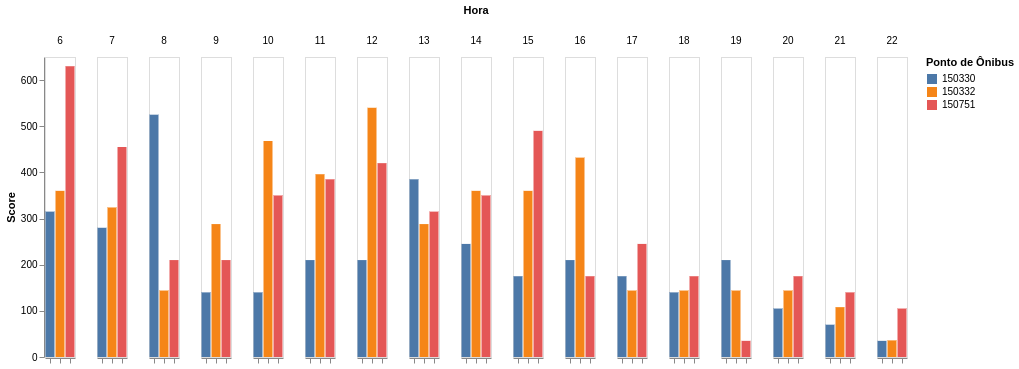
\includegraphics[width=.9\textwidth]{Capitulo4/img/centralidade-grau-rede-dinamica.png}
\caption{Centralidade de Grau da rede dinâmica - Dia 07/03/2019}
\label{fig:centralidade-grau-rede-dinamica}
\end{figure}



\begin{figure}
\centering
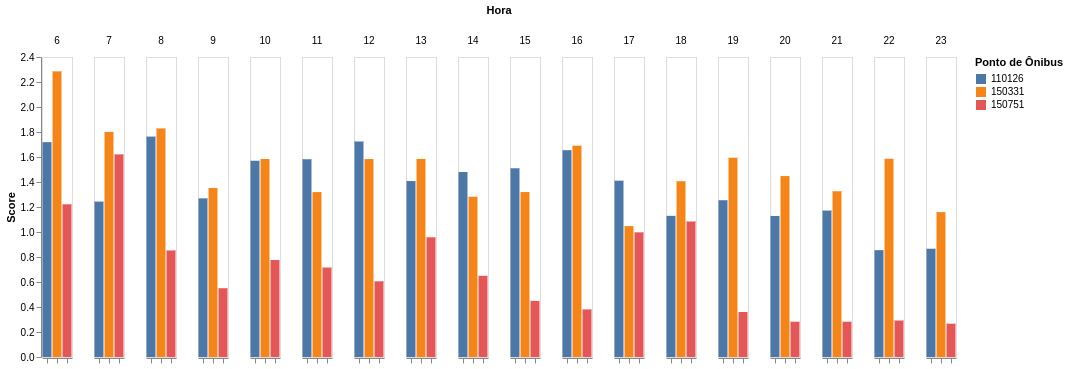
\includegraphics[width=.9\textwidth]{Capitulo4/img/pagerank-rede-dinamica.png}
\caption{Pagerank da rede dinâmica - Dia 07/03/2019}
\label{fig:pagerank-rede-dinamica}
\end{figure}


As medidas de comprimento das linhas da rede estática de transporte resultaram em 40~m, 38,14~km e 9,03~km para os comprimentos mínimo, máximo e médio (com desvio padrão de 6,5~km) das linhas de ônibus.

Já as medidas baseadas em caminhos mínimos entre pontos da rede resultaram em um valor mínimo de 2,5~m, diâmetro da rede (caminho mínimo mais longo) de 37.5~km e um percurso médio de 12~km. 

Estes caminhos mínimos foram obtidos através dos atributos de distância (\texttt{DISTANCE}) das arestas \texttt{NEXT\_STOP}, gerando uma rede ponderada do sistema de transporte de Curitiba. Note que esse percurso médio pode ou não ser factível com troca de ônibus (baldeação), dependendo da origem e destino do passageiro.
Tais métricas são úteis para comparação entre sistemas de transporte de diferentes cidades, e para planejamento do próprio sistema, seja na redução de distância ou no tempo de percurso dos passageiros.

% {\bf Resultado 5:} Tabela de medidas da rede estática: comprimento mínimo, máximo e médio das linhas (em km); média dos caminhos mínimos (de cada nó para todos os outros; diâmetro da rede (caminho mínimo mais longo);


 
%\ric{Cada resultado precisa ser explicado.}

% A Figura~\ref{fig:centralidade-grau-estatica} mostra a centralidade de grau considerando apenas os pontos de ônibus (rede estática, ou seja, sem movimentação de ônibus). Os pontos 150331, 110026 e 150332 são os pontos de maior centralidade de grau, ou seja, conectam um número maior de pontos de ônibus devido a um maior número de linhas que passam por estes pontos. Em Curitiba, enquanto que o segundo ponto localiza-se na região central da cidade, os dois outros pontos (150331 e 150332) localizam-se na região sul da cidade. Em todos os casos, são pontos para onde convergem várias linhas de ônibus antes de chegarem a terminais importantes da cidade (terminal Pinheirinho ao sul, nos caso dos pontos 150331 e 150332, e praça Rui Barbosa no centro, no caso do ponto 110026). 
%Cabe ressaltar que a rede complexa construída considera pontos distintos, mesmo em terminais de ônibus, seguindo representação da URBS.

%{\bf Resultado 1:} Grau dos nós (\emph{Bus Stop}) para a rede estática (sem \emph{Stops}) na forma de histograma para os 10 nós de maior grau;

 
% A Figura~\ref{fig:centralidade-grau-dinamica} mostra a centralidade de grau considerando as paradas de ônibus nos pontos de ônibus ao longo do dia (rede dinâmica, ou seja, com movimentação de ônibus). São mostrados os resultados para os três pontos de maior centralidade de grau da rede estática (150331, 110026 e 150332). Nota-se uma maior concentração no período da manhã e meio do dia, com diminuição gradual até o final da noite. Ao mesmo tempo, o ponto 150331 atende um elevado número de ônibus no período da manhã e no final da tarde. Essa última característica ocorre em Curitiba por conta do encerramento de atividades em empresas (trabalhadores retornando a suas casas) e estudantes de ensino noturno se deslocando para instituições de ensino.

 

% A Figura~\ref{fig:pagerank} mostra o \emph{page rank} considerando apenas a rede estática (pontos de ônibus). Os pontos 150331, 110026 e 110016 são os pontos de maior \emph{page rank}. Estes pontos se localizam, respectivamente, na região sul da cidade (na saída do terminal Pinheirinho), na região que conecta o centro a região nordeste da cidade (na direção de terminais Cabral, Boa Vista e Santa Cândida), nas proximidades do centro da cidade. Todos esses pontos conectam várias linhas que se afastam (pontos 150331 e 110126) ou se aproximam (ponto 11016) de regiões de grande concentração de pontos finais de linhas de ônibus. Ou seja, a importância destes pontos se deve a ligações com outros pontos importantes (pontos ou terminais com grande concentração de linhas).

%Lembrando que esta métrica indica relevância de pontos em relação aos demais pontos que se conectam a eles: são pontos importantes porque outros pontos significativos estão conectados, por linhas de ônibus, a eles.}

%{\bf Resultado 3:} \emph{PageRank} dos nós (\emph{Bus Stop}) para a rede estática (sem \emph{Stops}) na forma de histograma para os 10 nós de maior \emph{rank};

% \begin{figure}
% \centering
% \includegraphics[width=.9\textwidth]{fig/fig8.png}
% \caption{\emph{Page rank} para pontos de ônibus (dez maiores) sem movimentação de ônibus (rede estática).}
% \label{fig:pagerank}
% \end{figure}

%%%% Comentado por falta de espaço

% A Tabela~\ref{tab:n_linhas} mostra a comparação entre os três vértices de maior centralidade de grau (150332, 150331 e 110026) e os três vértices de maior \emph{page rank} (150331,150751,160244). \mar{Assim que os valores de grau forem recolocados, cabe um comentário sobre relação grau x page rank.}

% \begin{table}[h]
%     \caption{Comparação entre centralidade de grau  e \emph{page rank.}}
%     \label{tab:n_linhas}
%     \centering
%     \begin{tabular}{cccc} 
%         \hline
%         Ponto & Centralidade de grau & \emph{Page rank} \\
%         \hline
%         150332 & 63  & 4.15 \\
%         110026 & 64  &  3.75 \\
%         150751 & 63  & {\bf 5.53 } \\
%         150331 & 65  & {\bf 6.58} \\
%         160244 & 40  & {\bf4.82} \\
%         150330 &  32 &  4.75 \\
%         \hline 
        
%     \end{tabular}
% \end{table}

% \begin{table}[h]
%     \caption{Comparação entre Centralidade de grau  e \emph{page rank.}}
%     \label{tab:n_linhas}
%     \centering
%     \begin{tabular}{ccccc} 
%         \hline
%         Ponto & No. linhas & Centralidade de Grau & \emph{Page Rank} \\
%         \hline
%         110026 & 27  & 23 &  3.91 \\
%         150332 & 24  & 32 & 2.21 \\
%         150331 & 24  & 27 & {\bf 6.01} \\
%         110126 & 18  & 21 &  {\bf 5.50} \\
%         110016 & 16  & 11 & {\bf 4.57}\\
        
%         \hline  
%     \end{tabular}
% \end{table}



% A Figura~\ref{fig:betweeness} mostra a centralidade de intermediação considerando apenas a rede estática (pontos de ônibus). Os pontos 170154, 170085 e 170083 são os pontos de maior centralidade de intermediação. Estes pontos localizam-se na vizinhança do terminal Pinheirinho, localizado na parte sul de Curitiba, comportando-se como um \emph{hub} por onde passam percursos mais curtos entre pontos de ônibus da rede. Note também que esses percursos podem ou não ser factíveis com trocas de ônibus.
%Eles refletem indiretamente a movimentação de pessoas dessa região da cidade (basicamente bairros-dormitórios) para trabalharem ou estudarem nas demais partes da cidade, ou seja, a uma relação desses resultados com a evolução urbana da cidade.



\section{Integração temporal}


% Integração Temporal
% Os passageiros do transporte coletivo de Curitiba têm diferentes tipos de integração temporal para trocar de linha de ônibus ou de estação-tubo sem precisar pagar nova tarifa. Em 2017 foram mais de 600 mil usos nas integrações temporais das linhas urbanas da capital. Se contar o acesso às Ruas da Cidadania, esse atendimento sobe para quase um milhão.

% A proposta das integrações temporais no transporte é oferecer uma alternativa aos passageiros que ainda não têm acesso à integração no sistema. No transporte da capital, uma pessoa embarca num ponto e percorre todos os 21 terminais e as mais de 300 estações-tubo pagando apenas uma tarifa. Isso ocorre em 92\% da rede de transporte da cidade. A integração temporal busca complementar gradativamente essa rede.

% O único critério para usar a integração temporal é ter o cartão-transporte da URBS, que permite também o acesso às Ruas da Cidadania, onde o passageiro economiza uma tarifa no retorno ao ônibus. Veja quais são os tipos de integrações possíveis:

% Para o usuário ter direito à integração temporal, o mesmo deve utilizar o cartão-transporte da URBS em um dos validadores do Sistema de Transporte Coletivo de Curitiba (Ônibus, Terminal, Estação-Tubo), realizando assim um debito de passagem do seu Cartão Transporte e conforme as regras abaixo.

% OBS.: apenas os cartões-transporte nas modalidades Usuário e Estudante realizam integração temporal. Com o cartão-transporte Avulso não há a possibilidade de uso do benefício da integração temporal.

%%%%%% O que está abaixo não necessariamente permanecerá no texto - por enquanto é apenas uma referência para a seção


\begin{table}[htb]
    \caption{Valores dos parâmetros da análise de integração temporal.}
    \centering
    \begin{tabular}{lc} 
        \hline
        Parâmetro & Valor\\
        \hline
        Tamanho da janela & 10~min \\
        Passo da janela & 1~min \\
        Raio do cluster & 600~m  \\
        Separação entre clusters  & 1,2~km \\
        \hline  
    \end{tabular}
    \label{tab:parv}
\end{table}


% \ric{Resultados a serem apresentados sobre o levantamento de regiões candidatas para integração temporal:}

% \begin{itemize}
%     \item Visualização das regiões estudadas (centroides) no mapa de Curitiba;
    
%     \item Número de pontos e raio médio destas regiões, ou seja, os pontos selecionados estão em um raio muito menor do que 600~m?
    
%     \item Quantas linhas de ônibus servem cada região? Elas se conectam em algum outro ponto da rede, ou seja, existe um terminal ou estação tubo onde a transferência possa ser realizada sem pagamento de nova tarifa?
    
%     \item Dar especial atenção aos centroides que "integram" várias linhas (Alferes Poli?; Centro Cívico?); estes centroides, além de possuírem serviços "sincronizados" (precisa definir o que seria isso), permitem criar novas rotas;
    
% \end{itemize}

Para a análise da integração temporal, os pontos de ônibus com a maior quantidade de linhas são selecionados, conforme a proposta da Seção~\ref{sec:itemporal}. Estes pontos são apresentados na Tabela~\ref{tab:regioes-servico}. \ric{Exlicar os resultados da tabela e identificar em negrito quais pontos serão considerados como centroides da análise; explicar os critérios utilizados: efeito corredor; regiões próximas de terminais, etc.}

\ric{Padronizar no doc inteiro: \textit{nível de serviço} corresponde ao número de paradas de ônibus observadas nos pontos (quanto mais paradas, maior o nível de serviço; \textit{oferta de linhas} corresponde ao número de linhas que servem o ponto.}


% 110126	Rua Heitor S de Franca, 93	-25.423319	-49.268574	        84
% 180641	Av. Iguacu, 3064	-25.450068	-49.290573		            50
% 160245	Rua Mal. Otavio Saldanha Maza, 3046	-25.525816	-49.293896	59
% 120014	Av. Anita Garibaldi, 2393	-25.392260	-49.260983	        32

\begin{table}[htb]
    \caption{Centroides considerados.}
    \label{tab:regioes-servico}
    \centering
    \footnotesize
    \begin{tabular} {p{1.5cm}p{4.0cm}p{1.5cm}p{1.5cm}p{1.5cm}p{1.5cm}p{1.5cm}p{1.5cm} }  %%{clcccccc} 
        \hline
        Ponto (ID) & Endereço &Nº Méd. Veíc. & Desv. Pad. Veíc. &\# Linhas &Distância (m) & \# P Cluster &\# L Cluster  \\
        \hline
    \texttt{150332} &                       Rua Leon Nicolas, 2081  &              3.95 &                   2.03 &       32 &        331.00 &          16 &          59 \\
    \texttt{150751} &                  Av. Winston Churchill, 2677  &              3.67 &                   1.92 &       32 &        313.00 &          14 &          44 \\
    \texttt{150331} &                  Av. Winston Churchill, 2472  &              3.54 &                   1.78 &       33 &        414.00 &          15 &          76 \\
    \texttt{110024} &                        Rua Alferes Poli, 787  &              3.25 &                   1.64 &       31 &        407.00 &          15 &          56 \\
    \texttt{160244} &                       Rua Emanoel Voluz, 284  &              3.23 &                   1.60 &       22 &        476.00 &          13 &          58 \\
    \texttt{110026} &                        Rua Alferes Poli, 400  &              3.20 &                   1.69 &       32 &        430.00 &          15 &          66 \\
    \texttt{110022} &               Rua Vinte e Quatro de Maio, 280 &              3.10 &                   1.47 &       20 &        455.00 &          16 &          55 \\
    \texttt{150634} &                             Av. Iguacu, 2612  &              2.99 &                   1.34 &       18 &        417.00 &          13 &          40 \\
    \texttt{110120} &                    Av. Candido de Abreu, 707  &              2.96 &                   1.36 &       15 &        336.00 &          14 &          48 \\
    \textbf{\texttt{160245}} &          Rua Mal. Otavio Saldanha Maza, 3046  &              2.96 &                   1.24 &       16 &        426.00 &          13 &          59 \\
    \texttt{150330} &                  Av. Winston Churchill, 2546  &              2.95 &                   1.57 &       32 &        349.00 &          14 &          58 \\
    \textbf{\texttt{110126}} &                   Rua Heitor S de Franca, 93  &              2.94 &                   1.40 &       20 &        420.00 &          16 &          84 \\
    \texttt{140375} &                      Rua Leonardo Novicki, 8  &              2.83 &                   1.16 &        3 &        368.00 &           9 &           6 \\
    \texttt{150631} &                             Av. Iguacu, 1788  &              2.83 &                   1.34 &       18 &        456.00 &          13 &          34 \\
    \texttt{170051} &                       Rua Joaquim Sim?es, 10  &              2.79 &                   1.18 &       14 &        353.00 &          15 &          62 \\
    \texttt{110210} &               Av. Pres. Getulio Vargas, 1708  &              2.78 &                   1.36 &       20 &        462.00 &          10 &          42 \\
    \texttt{180535} &               Av. Pres. Getulio Vargas, 3047  &              2.74 &                   1.42 &       16 &        396.00 &          15 &          48 \\
    \textbf{\texttt{180641}} &                             Av. Iguacu, 3064  &              2.58 &                   1.22 &       13 &        427.00 &          14 &          50 \\
    \texttt{140228} &  Rua Engenheiro Benedito Mario da Silva, 570  &              2.56 &                   1.13 &        4 &        347.00 &          14 &          16 \\
    \texttt{108204} &                        Estac?o Vila S?o Pedro &              2.54 &                   1.59 &        4 &        344.00 &          14 &           7 \\
    \texttt{150635} &               Av. Pres. Getulio Vargas, 2676  &              2.51 &                   1.22 &       19 &        440.00 &          13 &          49 \\
    \texttt{120020} &                    Av. Anita Garibaldi, 3431  &              2.50 &                   1.17 &        9 &        373.00 &           8 &           9 \\
    \texttt{120403} &            Rua Lysimaco Ferreira da Costa, 1  &              2.46 &                   1.12 &       10 &        393.00 &          14 &          45 \\
    \texttt{110211} &               Av. Pres. Getulio Vargas, 1309  &              2.42 &                   1.22 &       20 &        426.00 &          14 &          65 \\
    \texttt{180534} &               Av. Pres. Getulio Vargas, 3355  &              2.42 &                   1.33 &       16 &        414.00 &          15 &          27 \\
    \texttt{110208} &                             Av. Iguacu, 1184  &              2.41 &                   1.13 &       18 &        385.00 &          14 &          78 \\
    \texttt{110037} &                        Av. Manoel Ribas, 531  &              2.37 &                   1.00 &        6 &        348.00 &          10 &          19 \\
    \textbf{\texttt{120014}} &                    Av. Anita Garibaldi, 2393  &              2.35 &                   1.15 &        6 &        354.00 &          11 &          32 \\
    \texttt{110033} &                        Av. Manoel Ribas, 530  &              2.34 &                   1.10 &       16 &        355.00 &           8 &          11 \\
    \texttt{103155} &                    Av. Candido de Abreu, 51   &              2.32 &                   1.19 &       19 &        446.00 &          16 &          72 \\
        \hline  
    \end{tabular}
\end{table}


    

% \begin{table}[htb]
%     \caption{Pontos de maior oferta de linhas.}
%     \label{tab:regioes-servico}
%     \centering
%     \footnotesize
%     \begin{tabular}{p{1.2cm}p{4.0cm}p{1.5cm}p{2.0cm}p{2.0cm}p{2.0cm}p{1.5cm} } 
%         \hline
%         \# Ponto & Endereço & Bairro &   Latitude &  Longitude &  Distância m. &  \# Linhas \\
%         \hline
% \texttt{110126} &                   Rua Heitor S de Franca, 93  &    Centro Civico & -25.423319 & -49.268574 &            420.0 &         84 \\
% \texttt{110208} &                             Av. Iguacu, 1184  &         Reboucas & -25.443296 & -49.272465 &            385.0 &         78 \\
% \texttt{150331} &                  Av. Winston Churchill, 2472  &       Cap?o Raso & -25.518349 & -49.295670 &            414.0 &         76 \\
% \texttt{103155} &                    Av. Candido de Abreu, 51   &    Centro Civico & -25.423600 & -49.270050 &            446.0 &         72 \\
% \texttt{110026} &                        Rua Alferes Poli, 400  &         Reboucas & -25.440706 & -49.271458 &            430.0 &         66 \\
% \texttt{110211} &               Av. Pres. Getulio Vargas, 1309  &         Reboucas & -25.445198 & -49.272274 &            426.0 &         65 \\
% \texttt{170051} &                       Rua Joaquim Sim?es, 10  &      Pinheirinho & -25.521141 & -49.296043 &            353.0 &         62 \\
% \texttt{150332} &                       Rua Leon Nicolas, 2081  &       Cap?o Raso & -25.515160 & -49.294445 &            331.0 &         59 \\
% \texttt{160245} &          Rua Mal. Otavio Saldanha Maza, 3046  &       Cap?o Raso & -25.525816 & -49.293896 &            426.0 &         59 \\
% \texttt{150330} &                  Av. Winston Churchill, 2546  &       Cap?o Raso & -25.519230 & -49.295456 &            349.0 &         58 \\
% \texttt{160244} &                       Rua Emanoel Voluz, 284  &      Pinheirinho & -25.524017 & -49.292990 &            476.0 &         58 \\
% \texttt{110024} &                        Rua Alferes Poli, 787  &         Reboucas & -25.443478 & -49.270140 &            407.0 &         56 \\
% \texttt{110022} &               Rua Vinte e Quatro de Maio, 280 &     350 - Centro & -25.439756 & -49.273240 &            455.0 &         55 \\
% \texttt{180641} &                             Av. Iguacu, 3064  &       Agua Verde & -25.450068 & -49.290573 &            427.0 &         50 \\
% \texttt{150635} &               Av. Pres. Getulio Vargas, 2676  &       Agua Verde & -25.449986 & -49.284863 &            440.0 &         49 \\
% \texttt{110120} &                    Av. Candido de Abreu, 707  &    Centro Civico & -25.418154 & -49.268750 &            336.0 &         48 \\
% \texttt{180535} &               Av. Pres. Getulio Vargas, 3047  &       Agua Verde & -25.451468 & -49.288750 &            396.0 &         48 \\
% \texttt{120403} &            Rua Lysimaco Ferreira da Costa, 1  &   Alto da Gloria & -25.417702 & -49.265144 &            393.0 &         45 \\
% \texttt{150751} &                  Av. Winston Churchill, 2677  &       Cap?o Raso & -25.520731 & -49.295383 &            313.0 &         44 \\
% \texttt{110210} &               Av. Pres. Getulio Vargas, 1708  &         Reboucas & -25.446516 & -49.275787 &            462.0 &         42 \\
% \texttt{150634} &                             Av. Iguacu, 2612  &       Agua Verde & -25.448942 & -49.287533 &            417.0 &         40 \\
% \texttt{150631} &                             Av. Iguacu, 1788  &       Agua Verde & -25.445711 & -49.278720 &            456.0 &         34 \\
% \texttt{120014} &                    Av. Anita Garibaldi, 2393  &        Boa Vista & -25.392260 & -49.260983 &            354.0 &         32 \\
% \texttt{180534} &               Av. Pres. Getulio Vargas, 3355  &       Agua Verde & -25.452467 & -49.291256 &            414.0 &         27 \\
% \texttt{110037} &                        Av. Manoel Ribas, 531  &           Merces & -25.422483 & -49.284330 &            348.0 &         19 \\
% \texttt{140228} &  Rua Engenheiro Benedito Mario da Silva, 570  &           Cajuru & -25.469620 & -49.205890 &            347.0 &         16 \\
% \texttt{110033} &                        Av. Manoel Ribas, 530  &           Merces & -25.422354 & -49.284145 &            355.0 &         11 \\
% \texttt{120020} &                    Av. Anita Garibaldi, 3431  &     S?o Lourenco & -25.383070 & -49.261860 &            373.0 &          9 \\
% \texttt{108204} &                        Estac?o Vila S?o Pedro &              NaN & -25.506739 & -49.284473 &            344.0 &          7 \\
% \texttt{140375} &                      Rua Leonardo Novicki, 8  &           Cajuru & -25.467724 & -49.198490 &            368.0 &          6 \\
%         \hline  
%     \end{tabular}
% \end{table}



\begin{figure}[!h]
\caption{Áreas de estudo para integração temporal.}
\label{fig:areas-integracao-temporal}
\centering
\subfloat[Centroides considerados.]{
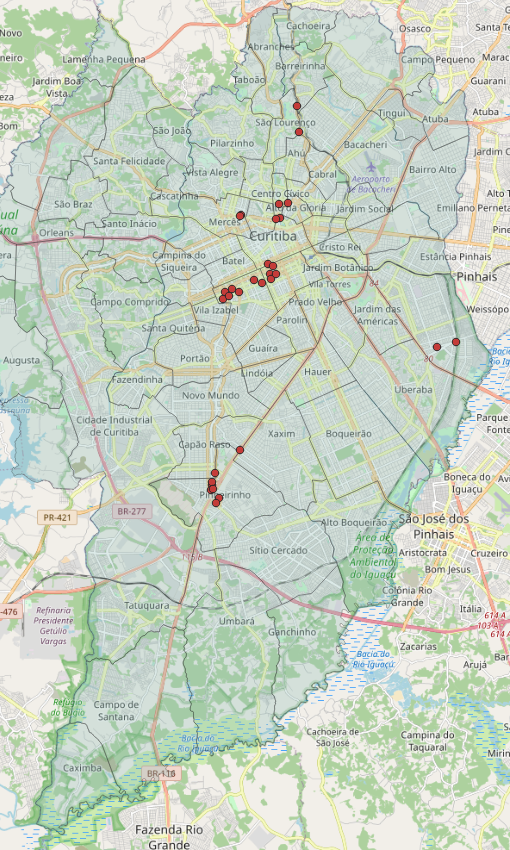
\includegraphics[width=.4\textwidth]{Capitulo4/img/areas-estudadas.png}
}
\quad
\subfloat[Centroides selecionados.]{
\label{fig:areas-integracao-sel}
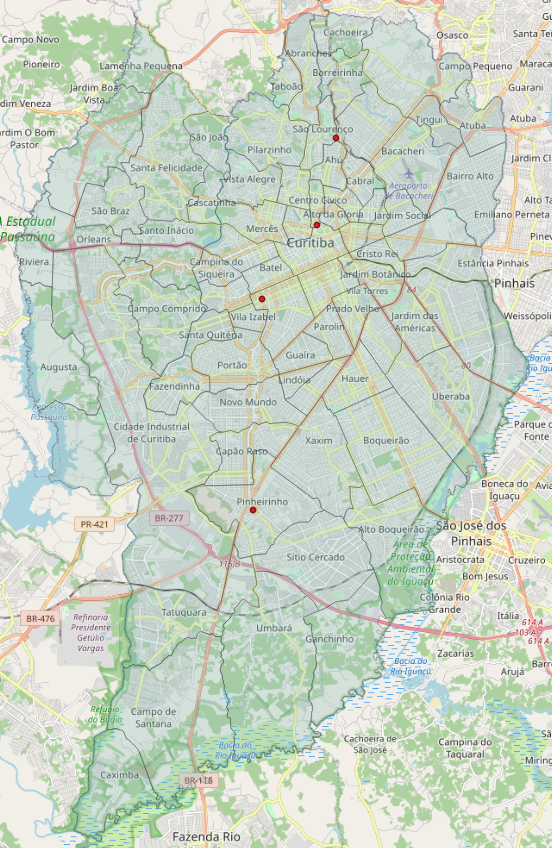
\includegraphics[width=.4\textwidth]{Capitulo4/img/map-centroide-areas-selecionadas.png}
}
\end{figure}

\ric{Agora precisa apresentar os resultados das correlações que permitem identificar os pontos dentro do cluster que serão considerados.}



% \begin{figure}
% \centering
% 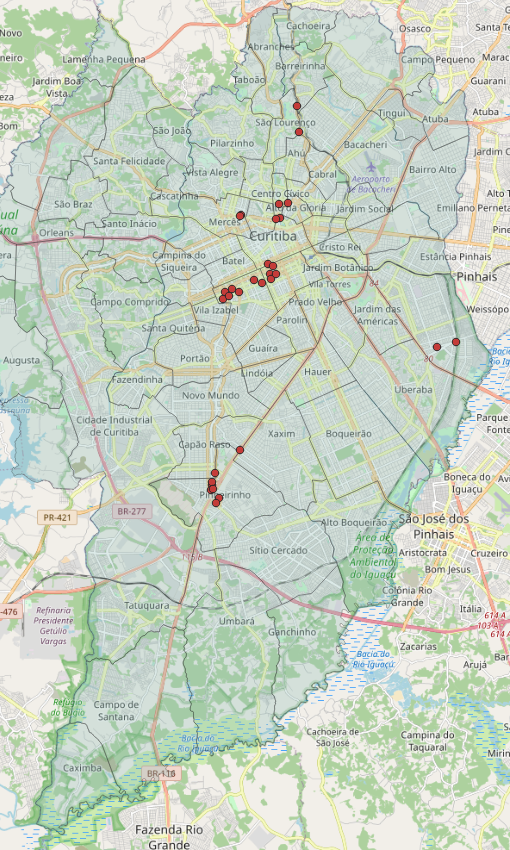
\includegraphics[width=.5\textwidth]{Capitulo4/img/areas-estudadas.png}
% \caption{Áreas de estudo para integração temporal}
% \label{fig:areas-integracao-temporal}
% \end{figure}

 

% \ric{Resultados a serem apresentados sobre o impacto na rede da implementação da integração temporal para as regiões selecionadas:}

% \begin{itemize}
%     \item Tem impacto na métrica de redes complexas (centralidade de proximidade ou intermediação, diâmetro)?
% \end{itemize}

A Tabela~\ref{tab:centralidade-proximidade-rede-estatica-integracao-temporal} mostra as alterações no diâmetro da rede (maior caminho mínimo na entre dois pontos da rede) e no caminho mínimo médio da rede (média dos caminhos mínimos da rede).

\begin{table}[htb]
    \caption{Diâmetro e caminho mínimo médio da rede antes e depois da integração temporal.}
    \label{tab:centralidade-proximidade-rede-estatica-integracao-temporal}
    \centering
    \footnotesize
    \begin{tabular}{ccc} 
        \hline
        Rede & Diâmetro (km) & Média dos caminhos mínimos (km)\\
        \hline
           Sem integração &  37.481 &  12.242 \\
           Com integração &  37.085 &  12.117 \\
        \hline  
    \end{tabular}
\end{table}


\begin{figure}[!h]
\caption{Pagerank da rede estática antes e depois da integração temporal.}
\label{fig:map-pagerank-estatica-antes}
\centering
\subfloat[Pagerank (antes).]{
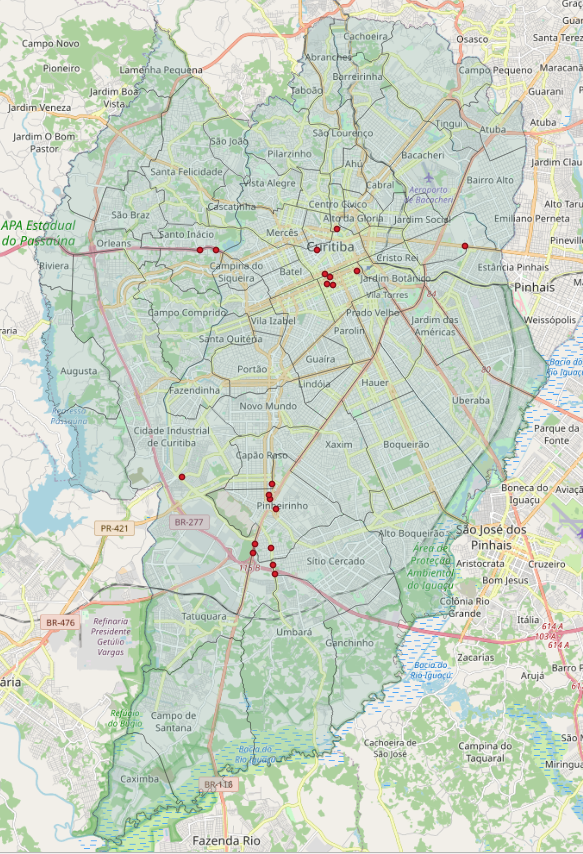
\includegraphics[width=.4\textwidth]{Capitulo4/img/rede-estatica/map-pagerank.png}
}
\quad
\subfloat[Pagerank (depois).]{
\label{fig:map-pagerank-estatica-depois}
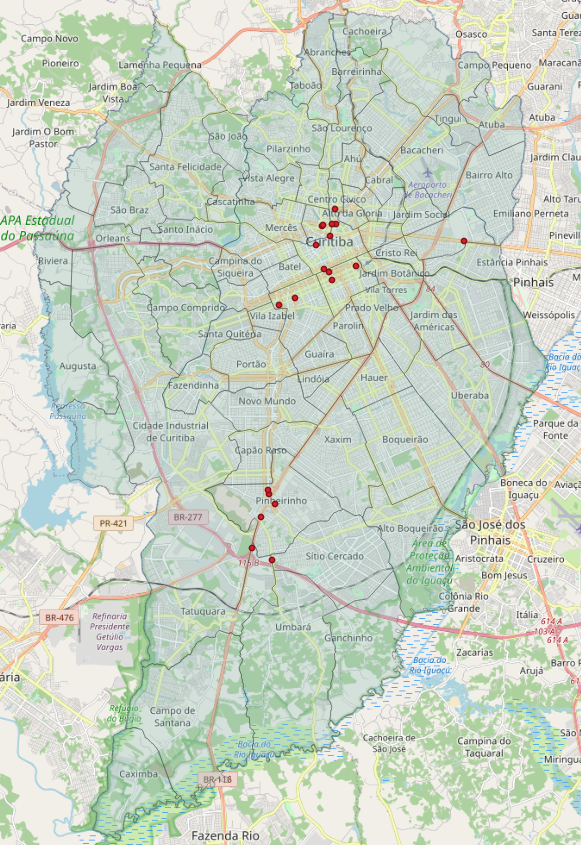
\includegraphics[width=.4\textwidth]{Capitulo4/img/rede-estatica/it-pagerank.png}
}
\end{figure}




\begin{table}[htb]
    \caption{Pontos de ônibus com maior pagerank da rede estática - INTEGRAÇÃO TEMPORAL.}
    \label{tab:pagerank-rede-estatica-integracao-temporal}
    \centering
    \footnotesize
    \begin{tabular}{p{1.0cm}p{8.0cm}p{3.0cm} } 
        \hline
        Número & Endereço  & Score \\
        \hline
           \texttt{110126} &          Rua Heitor S de Franca, 93 - Centro Civico &   6.259626 \\
           \texttt{110120} &           Av. Candido de Abreu, 707 - Centro Civico &   4.304215 \\
           \texttt{110016} &                      Rua Cruz Machado, 301 - Centro &   4.273913 \\
           \texttt{160076} &  Rodovia BR476 - Pista Lateral, 20227 - Pinheirinho &   4.110950 \\
           \texttt{103155} &           Av. Candido de Abreu, 51  - Centro Civico &   4.110654 \\
           \texttt{150751} &            Av. Winston Churchill, 2677 - Cap?o Raso &   4.067117 \\
           \texttt{110133} &               Rua Trajano Reis, 296 - S?o Francisco &   3.965037 \\
           \texttt{110201} &             Rua Inacio Lustosa, 434 - S?o Francisco &   3.828120 \\
           \texttt{150635} &         Av. Pres. Getulio Vargas, 2676 - Agua Verde &   3.799496 \\
           \texttt{110122} &        Rua Bar?o do Serro Azul, 217 - S?o Francisco &   3.766129 \\
           \texttt{160145} &             Rua Nicola Pellanda, 1719 - Pinheirinho &   3.706153 \\
           \texttt{110024} &                    Rua Alferes Poli, 787 - Reboucas &   3.682419 \\
           \texttt{160072} &            Rodovia BR476, 21283 - Cidade Industrial &   3.668968 \\
           \texttt{130215} &        Av. Victor Ferreira do Amaral, 1447 - Tarum? &   3.627512 \\
           \texttt{150330} &            Av. Winston Churchill, 2546 - Cap?o Raso &   3.561869 \\
           \texttt{110022} &        Rua Vinte e Quatro de Maio, 280-350 - Centro &   3.558696 \\
           \texttt{110147} &              Rua Conselheiro Laurindo, 1264- Centro &   3.554745 \\
           \texttt{160244} &                Rua Emanoel Voluz, 284 - Pinheirinho &   3.539183 \\
           \texttt{180534} &         Av. Pres. Getulio Vargas, 3355 - Agua Verde &   3.442686 \\
           \texttt{110026} &                    Rua Alferes Poli, 400 - Reboucas &   3.437565 \\
        \hline  
    \end{tabular}
\end{table}


   
\begin{figure}[!h]
\caption{Centralidade de intermediação da rede estática antes e depois da integração temporal.}
\label{fig:map-betweeness-rede-estatica-antes}
\centering
\subfloat[Centralidade de intermediação (antes).]{
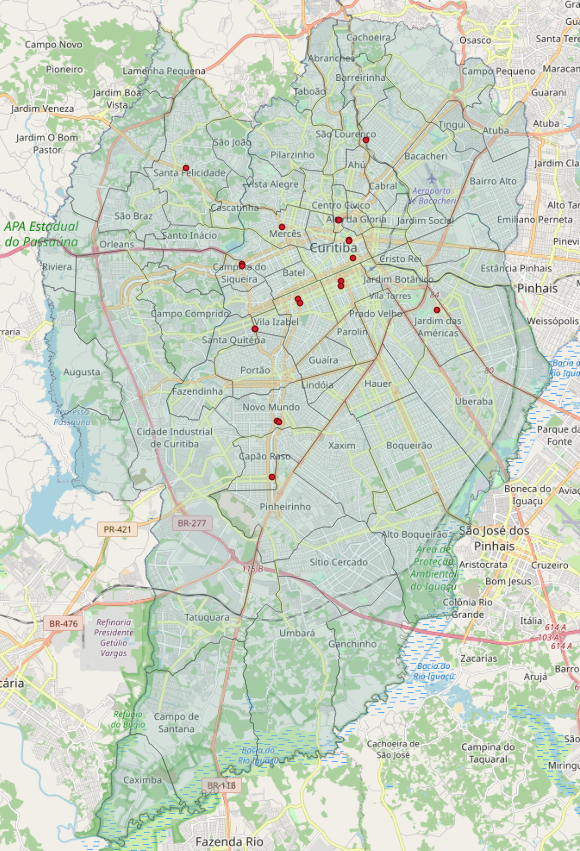
\includegraphics[width=.4\textwidth]{Capitulo4/img/rede-estatica/map-centralidade-intermediacao.png}
}
\quad
\subfloat[Centralidade de intermediação (depois).]{
\label{fig:map-betweeness-rede-estatica-depois}
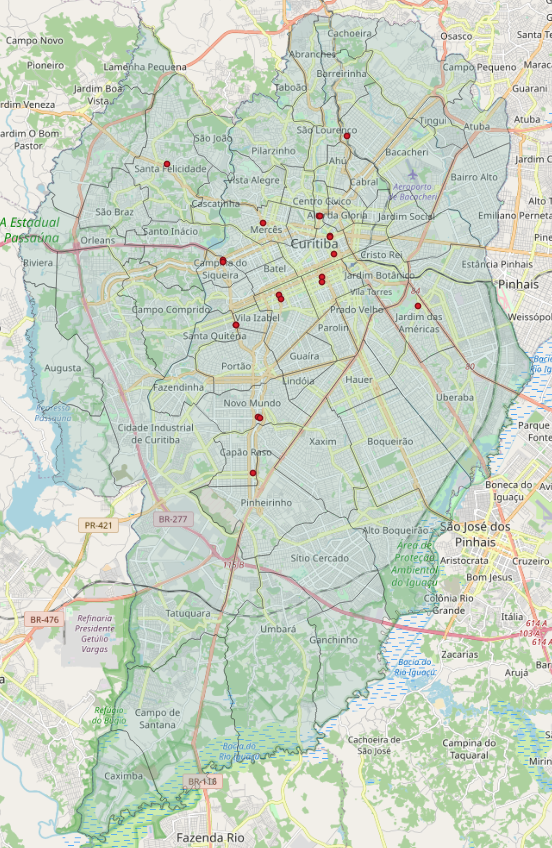
\includegraphics[width=.4\textwidth]{Capitulo4/img/rede-estatica/it-centralidade-intermediacao.png}
}
\end{figure}


\begin{table}[htb]
    \caption{Pontos de maior centralidade de intermediação da rede estática - INTEGRAÇÃO TEMPORAL.}
    \label{tab:centralidade-intermediação-rede-estatica-integracao-temporal}
    \centering
    \footnotesize
    \begin{tabular}{p{1.0cm}p{8.0cm}p{3.0cm} } 
        \hline
        Número & Endereço  & Score \\
        \hline
       \texttt{109093} &       Terminal Capão Raso - 023 - Inter 2 (Anti-Horario) / 508-Sitio Cercado (Anti-Horario)  & 6855318.96 \\
       \texttt{109003} &                                                            Estacão Tubo Agua Verde / Iguacu  & 6807440.93 \\
       \texttt{109067} &                                                                 Estacão Tubo Santa Quiteria  & 5405425.10 \\
       \texttt{109023} &                                                             Estacão Tubo Comendador Fontana  & 5382498.67 \\
       \texttt{109004} &                                                                            Estacão Tubo Ahu  & 5336610.11 \\
       \texttt{109073} &                                                            Estacão Tubo Westphalen / Iguacu  & 5272750.15 \\
       \texttt{109066} &                                                                 Estacão Tubo Santa Quiteria  & 5043475.18 \\
       \texttt{109018} &                                                                Estacão Tubo Circulo Militar  & 4862068.29 \\
       \texttt{109019} &                                                                Estacão Tubo Circulo Militar  & 4717134.35 \\
       \texttt{109098} &                                 Terminal Pinheirinho - 508 - Sitio Cercado (Anti - Horario)  & 4577417.96 \\
       \texttt{109167} &  Terminal Campina do Siqueira - 023 - Inter 2 (Anti-Horario) - 024 - C.Raso - Camp.Siqueira  & 4528242.96 \\
       \texttt{109121} &                             Terminal Santa Felicidade - 307 - Santa Felicidade/ Bairro Alto  & 4132291.61 \\
       \texttt{109022} &                                                             Estacão Tubo Comendador Fontana  & 3991819.60 \\
       \texttt{109125} &                                      Terminal Campina do Siqueira - 022 - Inter 2 (Horario)  & 3956243.75 \\
       \texttt{109034} &                                                            Estac?o Tubo Jardim das Americas  & 3906475.77 \\
       \texttt{109046} &                                                                         Estacão Tubo Merces  & 3788064.92 \\
       \texttt{109002} &                                                    Estacão Tubo Agua Verde / Getulio Vargas  & 3715861.15 \\
       \texttt{109074} &                                                    Estacão Tubo Westphalen / Getulio Vargas  & 3715837.15 \\
       \texttt{109030} &                                                                      Estacão Tubo Guadalupe  & 3715813.15 \\
       \texttt{109097} &                       Terminal Capão Raso - 507 - Sitio Cercado(H) - 610-S.Cercado / C.Raso  & 3706962.79 \\
        \hline  
    \end{tabular}
\end{table}




\begin{figure}[!h]
\caption{Centralidade de proximidade da rede estática antes e depois da integração temporal.}
\label{fig:map-closeness-rede-estatica-antes}
\centering
\subfloat[Centralidade de proximidade (antes).]{
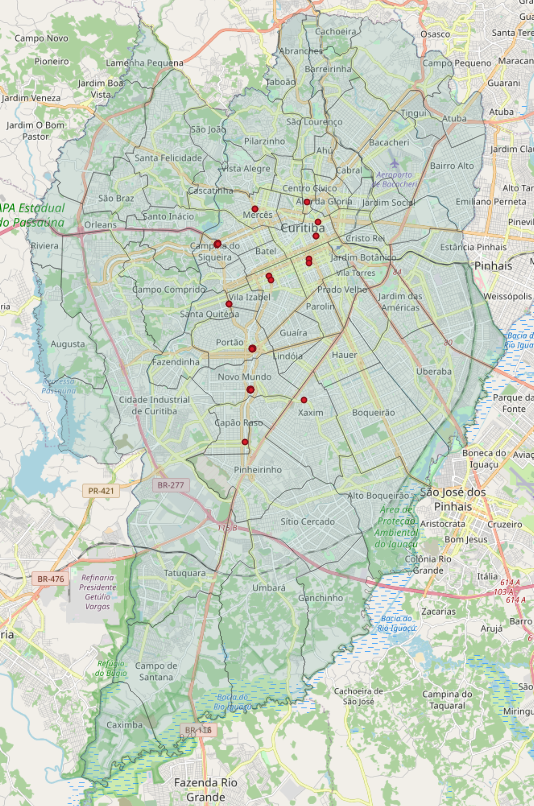
\includegraphics[width=.4\textwidth]{Capitulo4/img/rede-estatica/map-centralidade-proximidade.png}
}
\quad
\subfloat[Centralidade de proximidade (depois).]{
\label{fig:map-closeness-rede-estatica-depois}
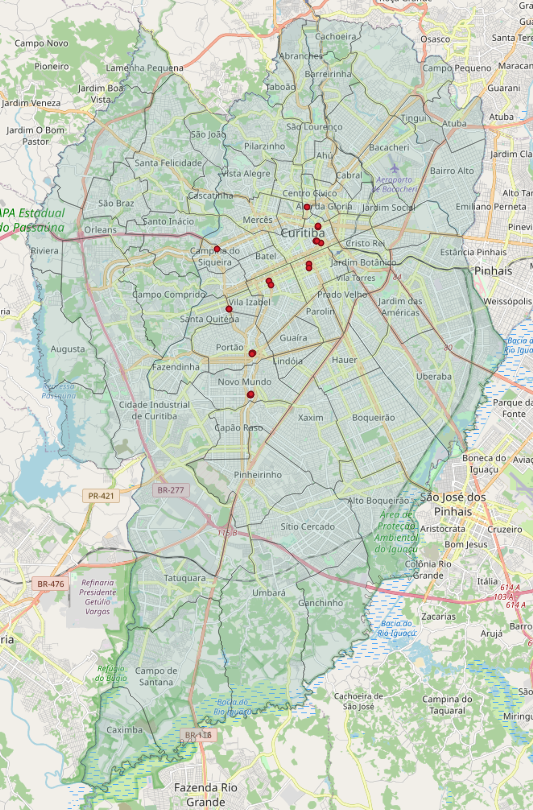
\includegraphics[width=.4\textwidth]{Capitulo4/img/rede-estatica/it-centralidade-proximidade.png}
}
\end{figure}

   
\begin{table}[htb]
    \caption{Pontos de maior centralidade de proximidade da rede estática - INTEGRAÇÃO TEMPORAL.}
    \label{tab:centralidade-proximidade-rede-estatica-integracao-temporal}
    \centering
    \footnotesize
    \begin{tabular}{p{1.0cm}p{9.0cm}p{3.0cm} } 
        \hline
        Número & Endereço & Score \\
        \hline
            \texttt{109003} &                                                            Estac?o Tubo Agua Verde / Iguacu &  0.093 \\
           \texttt{109093} &       Terminal Cap?o Raso - 023 - Inter 2 (Anti-Horario) / 508-Sitio Cercado (Anti-Horario)  &  0.092 \\
           \texttt{109073} &                                                            Estac?o Tubo Westphalen / Iguacu  &  0.091 \\
           \texttt{109019} &                                                                Estac?o Tubo Circulo Militar  &  0.091 \\
           \texttt{109002} &                                                    Estac?o Tubo Agua Verde / Getulio Vargas  &  0.091 \\
           \texttt{109030} &                                                                      Estac?o Tubo Guadalupe  &  0.090 \\
           \texttt{109023} &                                                             Estac?o Tubo Comendador Fontana  &  0.090 \\
           \texttt{109097} &                       Terminal Cap?o Raso - 507 - Sitio Cercado(H) - 610-S.Cercado / C.Raso  &  0.090 \\
           \texttt{109067} &                                                                 Estac?o Tubo Santa Quiteria  &  0.090 \\
           \texttt{109018} &                                                                Estac?o Tubo Circulo Militar  &  0.090 \\
           \texttt{109074} &                                                    Estac?o Tubo Westphalen / Getulio Vargas  &  0.090 \\
           \texttt{109090} &                                                Terminal Port?o - 700 - Pinheirinho / Cabral  &  0.089 \\
           \texttt{109028} &                 Terminal Guadalupe - 702 - Caiua / Cachoeira - X36 - Fazendinha / Guadalupe  &  0.089 \\
           \texttt{109028} &                                             Terminal Guadalupe - 705-Fazendinha / Guadalupe  &  0.089 \\
           \texttt{109066} &                                                                 Estac?o Tubo Santa Quiteria  &  0.089 \\
           \texttt{109167} &  Terminal Campina do Siqueira - 023 - Inter 2 (Anti-Horario) - 024 - C.Raso - Camp.Siqueira  &  0.088 \\
           \texttt{109091} &                                                   Terminal Port?o - 022 - Inter 2 (Horario)  &  0.088 \\
           \texttt{109089} &                                              Terminal Port?o - 023 - Inter 2 (Anti-Horario)  &  0.088 \\
           \texttt{109095} &                                               Terminal Cap?o Raso - 022 - Inter 2 (Horario)  &  0.088 \\
           \texttt{109029} &        Terminal Guadalupe - 256 - Barreirinha / Guadalupe - 505 - Boqueir?o / Centro Civico  &  0.088 \\
                \hline  
    \end{tabular}
\end{table}


   

\ric{Seria possível fazer uma análise mais local de integração das linhas em cada cluster?. Por exemplo, quais horários ocorre melhor sincronização das linhas do cluster?}
 

\section{Sumário do capítulo}

\ric{Destacar os pontos principais do capítulo e eventuais ganchos com outros capítulos.}



